\section{Evaluation}
We compare the performance of this system with that of BPFS and ext4 file systems to evaluate its design and implementation. We use the performance of BPFS as a baseline and focus on following key questions:
\begin{itemize}
\item What is the cost and overhead of the anti caching mechanism on top of the BPFS system?
\item How does the degree of hotness and coldness of stored data affect the performance of the system?
\item How does this file system perform for different cache eviction threshold? (Improve this)
\end{itemize}

\subsection{Method}
Making a meaningful performance comparison of this system with both the memory based file system such as BPFS and the disk based file system such as ext4 presents presents challenges at different levels. We cannot make comparison in isolation since our implementation is a hybrid approach that incorporates both systems. Another difficulty is that for a disk based file systems, such as ext4 that runs in the kernel layer, several parameters and behaviors are opaque to users and we have very limited contol on enforcing the pure disk-based behaviors. For instance, ext4 filesystems performs several operations in memory and commit to the disk only periodically [cite{something}]. 

For the purpose of the evaluation, we run our experiments on a real hardware with 8 CPU cores running RedHat Linux Operating Systems with 16 GM of memory, 500 GB of Solid state Drive and * MB cacheline. We simulate the behavior of NVM on the DRAM due to unavailability of the hardware (really???). Unless otherwise noted, both the original and our implementation of BPFS are mounted in the memory with 2 GB image. The anticaching daemon is set to run at 10 ms by default with caching occupancy threshold of 40 MB. These values were chosen by performing emperical analysis.    

\subsection{Experimental evaluations}
In this section we present the experimental evaluations of this file system using differnt micro and macro benchmarks and throughput evalations and offer comparisons with those of BPFS and ext4 file-systems. 

\subsubsection{Microbenchmarks}
\begin{figure}
\centering
\vspace{-0.2in}
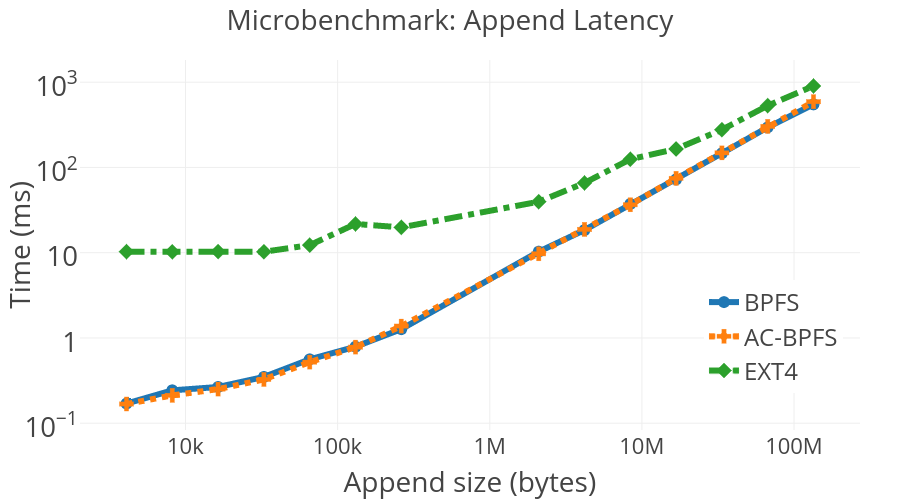
\includegraphics[width=0.5\textwidth]{figs/append.png}
\vspace{-0.2in}
\mycaption{fig-append}{Design Overview of BPFS}{\footnotesize The figure shows the overall design of our system. XXX}
\end{figure}



\begin{table}[!t]
%\vspace{0.1in}
\begin{center}
{\footnotesize
\begin{tabular}{c|c|l}
\textbf{Operations} & \textbf{Anti Cache BPFS(ms)} & \textbf{BPFS(ms)} \\
\hline
chmod&5.26&5.19 \\
create&6.49&6.45 \\
link&6.21&6.24 \\
mkdir&6.61&6.55 \\
read&4.67&4.61 \\
readdir&3.24&3.1 \\
rename\_dir\_intra&8.3&7.61 \\
rename\_file\_inter&8.6&7.82 \\
rmdir&6.66&5.95 \\
symlink&6.58&6.46 \\
unlink\_16M&10.03&10.42 \\
unlink\_hardlink&5.5&5.5 \\
write\_1M\_4k&6.91&6.22 \\

\end{tabular}
}
\end{center}
\vspace{-0.1in}
\mycaption{tbl-micro}{Microbenchmark}{\footnotesize The table
shows XXXX
}
\end{table}

\begin{figure}
\centering
\vspace{-0.2in}
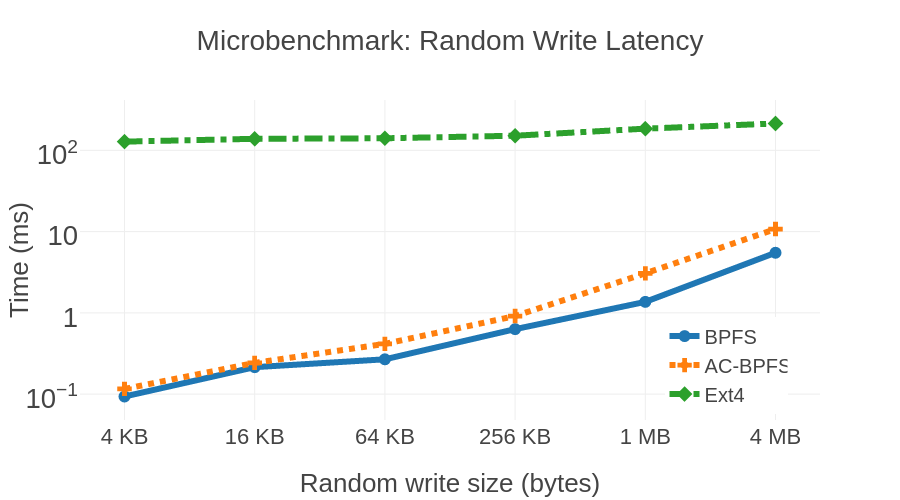
\includegraphics[width=0.5\textwidth]{figs/write.png}
\vspace{-0.2in}
\mycaption{fig-write}{Design Overview of BPFS}{\footnotesize The figure shows the overall design of our system. XXX}
\end{figure}


\begin{figure}
\centering
\vspace{-0.2in}
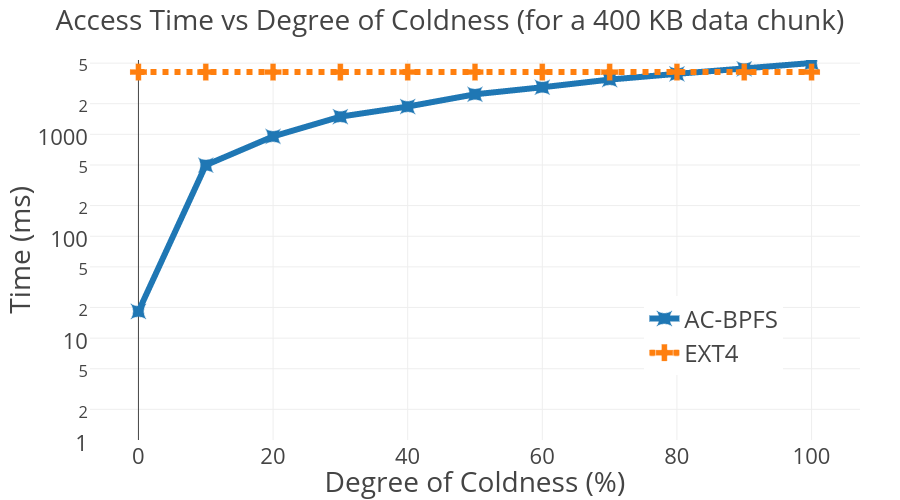
\includegraphics[width=0.5\textwidth]{figs/coldness.png}
\vspace{-0.2in}
\mycaption{fig-coldness}{Design Overview of BPFS}{\footnotesize The figure shows the overall design of our system. XXX}
\end{figure}


\subsubsection{Macrobenchmarks}

\begin{figure}
\centering
\vspace{-0.2in}
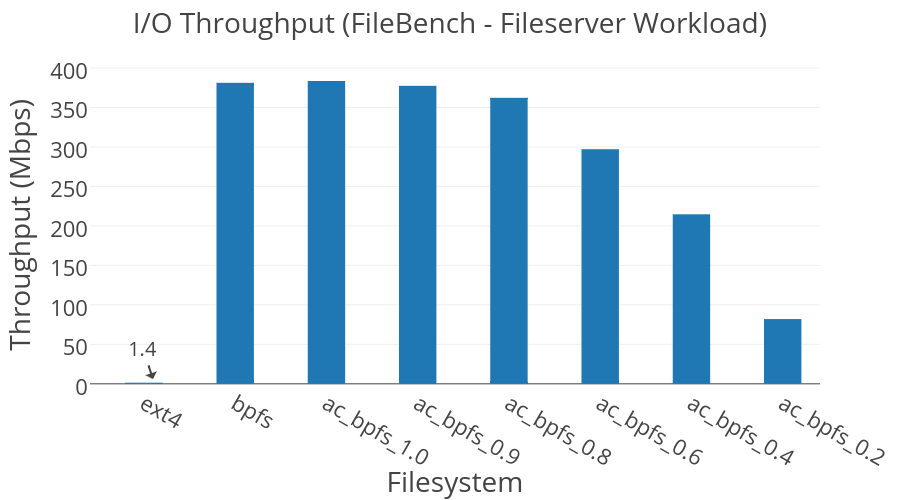
\includegraphics[width=0.5\textwidth]{figs/filebench.png}
\vspace{-0.2in}
\mycaption{fig-filebench}{Design Overview of BPFS}{\footnotesize The figure shows the overall design of our system. XXX}
\end{figure}

\begin{figure}
\centering
\vspace{-0.2in}
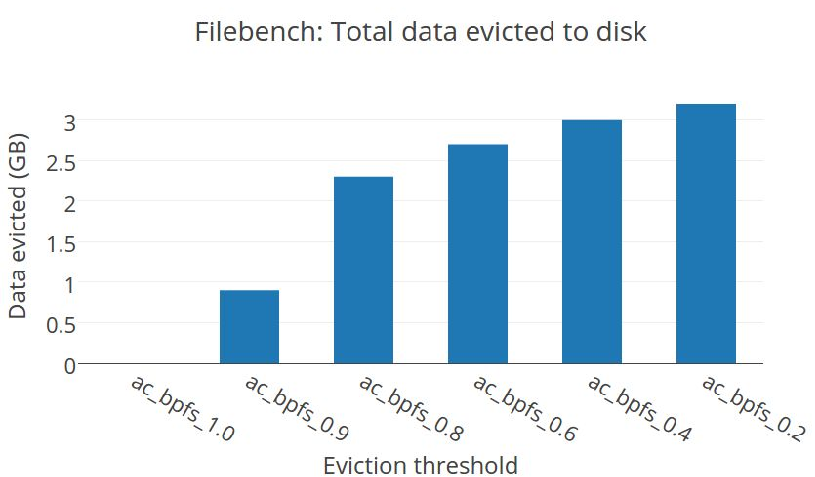
\includegraphics[width=0.5\textwidth]{figs/bench2.pdf}
\vspace{-0.2in}
\mycaption{fig-fb2}{Design Overview of BPFS}{\footnotesize The figure shows the overall design of our system. XXX}
\end{figure}
